\chapter{Dijkstra Algorithm with Data Structures}
\begin{algoprob}
	\problemtitle{Minimum Weight Path}
	\probleminput{Directed Graph $G=(V,E)$, $s\in V$ is source and $W=\{w_e\in \bbZ_+\colon e\in E\}$}
	\problemquestion{$\forall\ v\in V-\{s\}$ find minimum weight path $s\rightsquigarrow v$.}
\end{algoprob}

This is the problem we will discuss in this chapter. In this chapter we will often use the term `shortest distance' to denote the minimum weight path distance. One of the most famous algorithm for finding out minimum weight paths to all vertices from a given source vertex is Dijkstra's Algorithm
\section{Dijkstra Algorithm}
We will assume that the graph is given as adjacency list. Dijkstra Algorithm is basically dynamic programming. Suppose $\delta(v)$ is the shortest path distance from $s\rightsquigarrow v$.  Then we have the following relation:
$$\delta(v)=\min\limits_{u:(u,v)\in E}\{\delta(u)+e(u,v)\}$$And suppose for any vertex $v\in V-\{s\}$, $dist(v)$ be the distance from $s$ estimated by the algorithm at any point. This is why  Dijkstra's algorithm maintains a set $S$  of vertices   whose final shortest-path weights from the source $s$ have already been determined. The algorithm repeatedly selects the vertex $u\in V-S$ with minimum shortest-path estimate and estimates the distances of neighbors of $u$. So here is the algorithm:

\begin{algorithm}
	\SetKwComment{Comment}{// }{ }
	\DontPrintSemicolon
	\KwIn{Adjacency Matrix of digraph $G=(V,E)$, source vertex $s\in V$ and weight function $W=\{w_e\in \bbZ_+\colon e\in E\}$}
	\KwOut{$\forall\ v\in V-\{s\}$ minimum weight path from $s\rightsquigarrow v$}
	\Begin{
		$S\longleftarrow \emptyset$, $U\longleftarrow V$\;
		$dist(s)\longleftarrow 0$, $\forall\ v\in V-\{s\}$, $dist(v)\longleftarrow\infty$\;
		\While{$U\neq \emptyset$}{
			$u\longleftarrow \min\limits_{u\in U} dist(u)$ and remove $u$ from $U$\;
			$S\longleftarrow S\cup \{u\}$\;
			\For{$e=(u,v)\in E$}{$dist(v)\longleftarrow \min\{dist(v), dist(u)+w(u,v)\}$}
		}
	}
	\caption{\prb{Dijkstra}$(G,s,W)$}
\end{algorithm}

Here below we give an example of how the Dijkstra algorithm works:
%\begin{center}

\begin{figure}[h]
	\centering
	\begin{tikzpicture}[
			node distance = 12mm and 14mm,
			every state/.append style = {inner sep=0pt, fill=gray!10,
					minimum size=7mm},
			every edge/.style = {draw, -Stealth, bend angle=15},
			auto=right,
		]

		%
		%	\draw[blue!20, line width=5pt] 	(s1) to                     (s2);
		%
		\begin{scope}[shift={(-6,0)}]
			\node (s1) [state,fill=gray!30,label={left:$s$}]         {$\boldsymbol{0}$};
			\node (s2) [state, above right=of s1]   {$\boldsymbol{\infty}$};
			\node (s3) [state, right=of s2]         {$\boldsymbol{\infty}$};
			\node (s4) [state, below right =of s1]   {$\boldsymbol{\infty}$};
			\node (s5) [state, right=of s4]          {$\boldsymbol{\infty}$};
			\draw   (s1) edge [ "$10$"]             (s2)
			(s1) edge ["$5$"]						(s4)
			(s2) edge ["$1$"]             			(s3)
			(s2) edge [bend right, "$2$"]			(s4)
			(s3) edge [bend right, "$4$"] 			(s5)
			(s5) edge [bend right,"$6$"]  			(s3)
			(s5) edge [bend left=80,looseness=1.2,  "$7$", swap]	(s1)
			(s4) edge ["$2$"] 						(s5)
			(s4) edge ["$9$"]						(s3)
			(s4) edge [bend right, "$3$"]			(s2);
		\end{scope}

		\begin{scope}[shift={(0,0)}]
			\node (s1) [state,fill=gray!30,label={left:$s$},fill=black,text=white]         {$\boldsymbol{0}$};
			\node (s2) [state, above right=of s1]   {$\boldsymbol{10}$};
			\node (s3) [state, right=of s2]         {$\boldsymbol{\infty}$};
			\node (s4) [state,fill=gray!30, below right =of s1]   {$\boldsymbol{5}$};
			\node (s5) [state, right=of s4]          {$\boldsymbol{10}$};
			\draw[blue!20, line width=5pt] (s1) -- (s2);
			\draw[blue!20, line width=5pt] (s1) -- (s4);
			\draw   (s1) edge [ "$10$"]             			(s2)
			(s1) edge ["$5$"]									(s4)
			(s2) edge ["$1$"]             						(s3)
			(s2) edge [bend right, "$2$"]						(s4)
			(s3) edge [bend right, "$4$"] 						(s5)
			(s5) edge [bend right,"$6$"]  						(s3)
			(s5) edge [bend left=80,looseness=1.2,"$7$", swap]	(s1)
			(s4) edge ["$2$"] 									(s5)
			(s4) edge ["$9$"]									(s3)
			(s4) edge [bend right, "$3$"]						(s2);

		\end{scope}

		\begin{scope}[shift={(6,0)}]
			\node (s1) [state,label={left:$s$},fill=black,text=white]         {$\boldsymbol{0}$};
			\node (s2) [state, above right=of s1]   {$\boldsymbol{8}$};
			\node (s3) [state, right=of s2]         {$\boldsymbol{13}$};
			\node (s4) [state, below right =of s1,fill=black,text=white]   {$\boldsymbol{5}$};
			\node (s5) [state, right=of s4,fill=gray!30]          {$\boldsymbol{7}$};
			\draw[red!20, line width=5pt] (s1) -- (s4);
			\draw[blue!20, line width=5pt] (s4) to [bend right=15] (s2);
			\draw[blue!20, line width=5pt] (s4) -- (s5);
			\draw[blue!20, line width=5pt] (s4) -- (s3);
			\draw   (s1) edge [ "$10$"]             			(s2)
			(s1) edge ["$5$"]									(s4)
			(s2) edge ["$1$"]             						(s3)
			(s2) edge [bend right, "$2$"]						(s4)
			(s3) edge [bend right, "$4$"] 						(s5)
			(s5) edge [bend right,"$6$"]  						(s3)
			(s5) edge [bend left=80,looseness=1.2,"$7$", swap]	(s1)
			(s4) edge ["$2$"] 									(s5)
			(s4) edge ["$9$"]									(s3)
			(s4) edge [bend right, "$3$"]						(s2);
		\end{scope}

		\begin{scope}[shift={(-6,-6)}]
			\node (s1) [state,fill=gray!30,label={left:$s$},fill=black,text=white]      {$\boldsymbol{0}$};
			\node (s2) [state,fill=gray!30, above right=of s1]   						{$\boldsymbol{8}$};
			\node (s3) [state, right=of s2]        		 								{$\boldsymbol{13}$};
			\node (s4) [state, below right =of s1,fill=black,text=white]   				{$\boldsymbol{5}$};
			\node (s5) [state, right=of s4,fill=black,text=white]          {$\boldsymbol{7}$};
			\draw[red!20, line width=5pt] (s1) -- (s4);
			\draw[red!20, line width=5pt] (s4) to [bend right=15] (s2);
			\draw[red!20, line width=5pt] (s4) -- (s5);
			\draw[blue!20, line width=5pt] (s5) to [bend right=15] (s3);
			\draw[blue!20, line width=5pt] (s5) to [bend left=80,looseness=1.3]	(s1);
			\draw   (s1) edge [ "$10$"]             			(s2)
			(s1) edge ["$5$"]									(s4)
			(s2) edge ["$1$"]             						(s3)
			(s2) edge [bend right, "$2$"]						(s4)
			(s3) edge [bend right, "$4$"] 						(s5)
			(s5) edge [bend right,"$6$"]  						(s3)
			(s5) edge [bend left=80,looseness=1.3,"$7$", swap]	(s1)
			(s4) edge ["$2$"] 									(s5)
			(s4) edge ["$9$"]									(s3)
			(s4) edge [bend right, "$3$"]						(s2);
		\end{scope}

		\begin{scope}[shift={(0,-6)}]
			\node (s1) [state,fill=gray!30,label={left:$s$},fill=black,text=white]         {$\boldsymbol{0}$};
			\node (s2) [state, above right=of s1,fill=black,text=white]   {$\boldsymbol{8}$};
			\node (s3) [state, right=of s2,fill=gray!30]         {$\boldsymbol{9}$};
			\node (s4) [state, below right =of s1,fill=black,text=white]   {$\boldsymbol{5}$};
			\node (s5) [state, right=of s4,fill=black,text=white]          {$\boldsymbol{7}$};
			\draw[red!20, line width=5pt] (s1) -- (s4);
			\draw[red!20, line width=5pt] (s4) to [bend right=15] (s2);
			\draw[red!20, line width=5pt] (s4) -- (s5);
			\draw[red!20, line width=5pt] (s5) to [bend right=15] (s3);
			\draw[blue!20, line width=5pt] (s2) -- (s3);
			\draw   (s1) edge [ "$10$"]             			(s2)
			(s1) edge ["$5$"]									(s4)
			(s2) edge ["$1$"]             						(s3)
			(s2) edge [bend right, "$2$"]						(s4)
			(s3) edge [bend right, "$4$"] 						(s5)
			(s5) edge [bend right,"$6$"]  						(s3)
			(s5) edge [bend left=80,looseness=1.3,"$7$", swap]	(s1)
			(s4) edge ["$2$"] 									(s5)
			(s4) edge ["$9$"]									(s3)
			(s4) edge [bend right, "$3$"]						(s2);
		\end{scope}

		\begin{scope}[shift={(6,-6)}]
			\node (s1) [state,fill=gray!30,label={left:$s$},fill=black,text=white]         {$\boldsymbol{0}$};
			\node (s2) [state, above right=of s1,fill=black,text=white]   {$\boldsymbol{8}$};
			\node (s3) [state, right=of s2,fill=black,text=white]         {$\boldsymbol{9}$};
			\node (s4) [state, below right =of s1,fill=black,text=white]   {$\boldsymbol{5}$};
			\node (s5) [state,fill=gray!30, right=of s4,fill=black,text=white]          {$\boldsymbol{7}$};
			\draw[red!20, line width=5pt] (s1) -- (s4);
			\draw[red!20, line width=5pt] (s4) to [bend right=15] (s2);
			\draw[red!20, line width=5pt] (s4) -- (s5);
			%	\draw[red!20, line width=5pt] (s5) to [bend right=15] (s3);	
			\draw[red!20, line width=5pt] (s2) -- (s3);
			\draw   (s1) edge [ "$10$"]             			(s2)
			(s1) edge ["$5$"]									(s4)
			(s2) edge ["$1$"]             						(s3)
			(s2) edge [bend right, "$2$"]						(s4)
			(s3) edge [bend right, "$4$"] 						(s5)
			(s5) edge [bend right,"$6$"]  						(s3)
			(s5) edge [bend left=80,looseness=1.3,"$7$", swap]	(s1)
			(s4) edge ["$2$"] 									(s5)
			(s4) edge ["$9$"]									(s3)
			(s4) edge [bend right, "$3$"]						(s2);
		\end{scope}
	\end{tikzpicture}
	\caption{The execution of Dijkstra’s algorithm. The source s is the leftmost vertex. The 	shortest-path estimates appear within the vertices, and shaded edges indicate predecessor values. Black vertices are in the set $S$ and at any iteration of while loop the shaded vertex has the minimum value. At any iteration the red edges are the edges considered in minimum weight path from $s$ using only vertices in $S$.}
\end{figure}

Suppose at any iteration $t$, let $dist_t(v)$ denotes the distance $v$ from $s$ calculated by algorithm for any $v\in V$ and $S^{(t)}$ denote the content of $S$ at $t^{th}$ iteration. In order to show that the algorithm correctly computes the distances we prove the following lemma:
\begin{Theorem}{}{}
	For each $v\in S^{(t)}$, $\dl(v)=dist_t(v)$ for any iteration $t$.
\end{Theorem}
\begin{proof}
	We will prove this induction. Base case is $|S^{(1)}|=1$. $S$ grows in size. Then only time $|S^{(1)}|=1$ is when $S^{(1)}=\{s\}$ and $d(s)=0=\dl(s)$. Hence, for base case this is correct.

	Suppose this is also true for $t-1$. Let at $t^{th}$ iteration the vertex $u\in V-S$ is picked. By induction hypothesis for all $v\in S^{(t)}-\{u\}$, $dist_t(v)=dist_{t-1}(v)=\dl(v)$. So we have to show that $dist_{t}(u)=\dl(u)$.

	Suppose for contradiction the shortest path from $s\rightsquigarrow u$ is $P$ and has total weight $=\dl(u)=w(P)<dist_t(u)$. Now $P$ starts with vertices from $S^{(t)}$ by eventually leaves $S$. Let $(x,y)$ be the first edge in $P$ which leaves $S$ i.e. $x\in S$ but $y\notin S$. By inductive hypothesis $dist_t(x)=\dl(x)$. Let $P_y$ denote the path $s\rightsquigarrow y$ following $P$. Since $y$ appears before $u$ we have $$w(P_y)=\dl(y)\leq \dl(u)=w(P)$$Now $$dist_t(y)\leq dist_t(x)+w(x,y)$$ since $y$ is adjacent to $x$. Therefore $$dist_t(y)\leq dist_t(x)+w(x,y)=\dl(y)\leq dist_t(y)\implies dist_t(y)=\dl(y)$$Now since both $u,y\notin S^{(t)}$ and the algorithm picked up $u$ we have $\dl(u)<dist_t(u)\leq dist_t(y)=\dl(y)$. But we can not have both $\dl(y)\leq \dl(u)$ and $\dl(u)<\dl(y)$. Hence contradiction. Therefore $\dl(u)=dist_t(u)$. Hence by mathematical induction for any iteration $t$, for all $v\in S^{(t)}$, $\dl(v)=dist_t(v)$.
\end{proof}

Therefore, by the lemma  after all iterations $S$ has all the vertices with their shortest distances from $s$ and henceforth the algorithm runs correctly.

Now in the algorithm there are two things which needed to keep track of. At every iteration of the while loop we needed to find the vertex $u$ which had the minimum distance from the source vertex, and we needed to update the distance of a vertex by decreasing the value as needed. So after the decrease we need to update the minimum distance vertex. So in any data structure used to do these two operations we need the following things:\begin{itemize}[label=$\bullet$]
	\item Need to store: $\forall\ v\in V$, $dist(v)$
	\item Operations: \begin{itemize}
		      \item \textsc{Extract-Min}: Gives the vertex with minimum distance in $v$ and remove from the data structure.
		      \item \textsc{Decrease-Key}: For vertex $v$ reduce $dist(v)$ to $k$.
	      \end{itemize}
\end{itemize}\parinf

In the algorithm we called \textsc{Extract-Min} $n$ times and \textsc{Decrease-Key} $m$ times.\parinn

\section{Data Structure 1: Linear Array}
So naively we can use a linear array of size $n$ where each element of the array corresponds to a vertex. Each element of the array is a tuple of flag of being in $U$ and the value $dist(v)$. To \textsc{Extract-Min} it takes $O(n)$ time since we need to compare all the elements and for \textsc{Decrese-Key} it takes $O(1)$ time. Therefore Dijkstra takes $n\cdot O(n)+O(m)=O(n^2)$ time.

\section{Data Structure 2: Min Heap}
A binary heap data structure is an array object that we can view as ``Almost complete binary'' tree (ACB tree). Each node of the tree corresponds to an element of the array. The tree is completely filled on all levels except possibly the lowest which is filled from the left up to a point.

Let the ACB tree has height $h$. Then heap  is completely field until height $h-1$ i.e. every vertex up to  level $h-2$ has exactly two children and a node at height $h-1$ is missing a child then:\begin{itemize}
	\item Either both children are missing or only right child are missing.
	\item Every vertex to the right of the node is missing both children.
\end{itemize}An ACB tree height $h$ is represented as an array of size $2^h-1$. For vertex $v$ stored at $A[i]$, the left child of $A$ is at $A[2i]$ and the right child is at $A[2i+1]$ and the parent of $A$ is at $A\lt[\lfloor\frac{i}{2}\rfloor\rt]$.
\begin{figure}[h!]
	\centering
	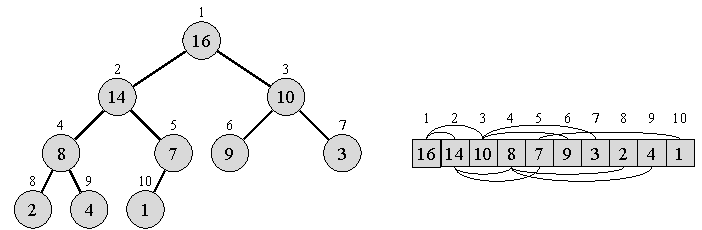
\includegraphics[width=0.9\textwidth]{images/Heap.pdf}
	\caption{A max-heap viewed as an ACB tree (left) and as an array (right)}
\end{figure}

Here we will study min-heap where the value of the children is more than the value of its parent.
\subsection{Initialization}
We create an array $A$ of size $n$. Initially we store the key value of every node to be $\infty$. And for the root $s$ we store $s.\emph{key}=0$.
\subsection{Extracting the Minimum}
For minimum, we already know the root of the heap or the first element of $A$ is the minimum. But after extracting the minimum we need to balance the heap so that it gets the properties of min-heap back. For that we replace the root with the right most element in the array $A$. Then balance the heap by moving it down if one of the child has \emph{key} smaller than \emph{node.key} and keep doing it until both child is larger.
\begin{algorithm}[]
	\caption{\textsc{Extract-Min}$(A)$}
	\SetKwComment{Comment}{// }{}
	\DontPrintSemicolon
	$t\longleftarrow A.\emph{size}$\;
	$Minval\longleftarrow A[1].\emph{key}$\;
	$A[1]\longleftarrow A[t]$\;
	$t\longleftarrow t-1$, $i\longleftarrow 1$\;
	\While{True}{
		\If{$2i\leq t$}{
			$left-val\longleftarrow A[2i].\emph{key}$\;
		}
		\Else{
			\Return{$minval$}\Comment*{No left child i.e. already at leaf}
		}
		\If{$2i+1\leq t$}{
			$right-val\longleftarrow A[2i+1].\emph{key}$
		}
		\Else{
			$right-val\longleftarrow \infty$\Comment*{No right child}
		}
		\If{$left-val\leq right-val$ and $A[i].\emph{key}<left-val$}{
			$curr\_elm\longleftarrow A[i]$\;
			$A[i]\longleftarrow A[2i]$\;
			$U[2i]\longleftarrow curr\_elm$\;
			$i\longleftarrow 2i$
		}
		\ElseIf{$right-val<left-val$}{
			$curr\_elm\longleftarrow A[i]$\;
			$A[i]\longleftarrow A[2i+1]$\;
			$U[2i+1]\longleftarrow curr\_elm$\;
			$i\longleftarrow 2i+1$
		}
		\Else{
			Break
		}
		\Return{$minval$}
	}
\end{algorithm}

In this algorithm for extracting min each time the height of the new root node increases by one at each iteration of the while loop. Hence, this takes at most $O(\log n)$ time.
\subsection{Decreasing Key of a Node}
After decreasing the \emph{key} of a node it may have smaller key than it's parent node. So move it upward i.e. replace with its parent node, and we keep doing it until the parent node has smaller value than it.
\begin{algorithm}[]
	\caption{\textsc{Decrease-Key}$(A,i,k)$}
	\DontPrintSemicolon
	$t\longleftarrow A.\emph{size}$\;
	$A[i]\longleftarrow k$\;
	\While{$i>1$ and $A[i].\emph{key}<A\lt[\lfloor\frac{i}{2}\rfloor\rt].\emph{key}$}{
		$curr\_elm\longleftarrow A[i]$\;
		$A[i].\emph{key}\longleftarrow A\lt[\lfloor\frac{i}{2}\rfloor\rt]$\;
		$A\lt[\lfloor\frac{i}{2}\rfloor\rt]\longleftarrow curr\_elm$\;
		$i\longleftarrow\lt\lfloor\frac{i}{2}\rt\rfloor$
	}
\end{algorithm}
Here again at each iteration of the while loop the height decreases by $1$. Hence, this takes at most $O(\log n)$ time.
\subsection{Time Complexity Analysis of Dijkstra}
Both \textsc{Extract-Min} and \textsc{Decrease-Key} takes $O(\log n)$ time for a min-heap. Now in a Dijkstra algorithm there are $n$ calls for \textsc{Extract-Min} and $m$ calls for \textsc{Decrease-Key}. Therefore, the total time taken by Dijkstra is $O(n\log n)+O(m\log n)=O(m\log n)$. But this is better when $m=o\lt(\frac{n^2}{\log n}\rt)$. Now we will show an improvement of min-heap where the amortized cost of \textsc{Extract-Min} is $O(\log n)$ and amortized cost of \textsc{Decrease-Key} is constant. But first we will take a detour of explaining amortized analysis.
\section{Amortized Analysis}
In amortized analysis, we average the time required to perform a sequence of data-structure operations over all the operations performed. With amortized analysis, we can show that the average cost of an operation is small, if we average over a sequence of operations, even though a single operation within the sequence might be expensive.
\nt{Amortized analysis in not average-case analysis as  amortized analysis guarantees the average performance of each operation in the worst case}

Consider the following algorithm:
\begin{algorithm}[]
	\caption{Amortized Analysis}
	\DontPrintSemicolon
	\KwIn{$n$}
	\Begin{
		$t\longleftarrow 0$, $X(0)\longleftarrow 0^n$\;
		\While{True}{
			$t\longleftarrow t+1$\;
			$X(t)\longleftarrow X(t-1)+1$
		}
	}
\end{algorithm}
Now the number of bit flips in this process is $1,2,1,3,\dots, n,\dots$. At any point the number of bit flips can be at most $n$. In the worst case an operation has cost $n$. We want to compute the average cost for an operation. We will show that starting from $X(0)=0^n$ the average cost is at most $2$. We will show 3 different proofs of this.
\begin{lemma}{}{}
	The total  cost of bit flips for $t$ operations is at most $2t$.
\end{lemma}
\begin{proofmany}{1 (Counting)}
	In $t$ operations:
	\begin{center}
		\begin{tabular}{rl}
			$n^{th}$ bit gets flipped:     & $t$ times                                                    \\
			$(n-1)^{th}$ bit gets flipped: & $\lfloor\frac{t}2\rfloor$ times (when $n^{th}$ bit is 1)     \\
			$(n-2)^{th}$ bit gets flipped: & $\lfloor\frac{t}4\rfloor$ times (when $(n-1)^{th}$ bit is 1) \\
			$\vdots$\hspace{1cm}           & \hspace{1cm}$\vdots$
		\end{tabular}
	\end{center}
	Therefore the total number of bit flips we get is $\leq t\lt(1+\frac12+\frac14+\cdots\rt)\leq 2t$.
\end{proofmany}

Now we will give a proof using the accounting method. In the accounting method of amortized analysis, we assign each operation an amortized cost that may differ from its actual cost. If the amortized cost is higher, the excess is stored as credit on data structure objects; if lower, credit is used to cover the gap. This way, expensive operations can be balanced by cheaper ones, and different operations may have different amortized costs.

\begin{proofmany}{2 (Charging)}
	Suppose every operation costs $2$ Rs. \begin{itemize}
		\item Every change from $0\to 1$ charges $1$ Rs and store $1$ Rs.
		\item Every change from $1\to 0$ charges $2$ Rs.
	\end{itemize}
	Now as you can see to change from $1\to 0$ that bit was previously changed from $0\to 1$. So to change from $1\to 0$ we can use the stored $1$ Rs. Hence, in average every operation costs exactly $0$ to $1$ Rs. Since there are $t$ operations total number of bit flips is at most $2t$.
\end{proofmany}

In the next proof we will analyze by computing a necessary potential function. After each operation we can calculate the potential difference.

\begin{proofmany}{3 (Potential)}
	Consider the potential function $\Phi(i)=\#$1's in $X(i)$. Let at $i^{th}$ operation $t_i$ bits were flipped from $1\to 0$. Now any operation flips at most $1$ bit from $0\to 1$. Therefore, number of bit flips in $i^{th}$ operation is at most $t_i+1$. Therefore, we have $$\Phi(i)\leq \Phi(i-1)-t_i+1$$since the number of $1$'s in $\Phi(i)$ is decreased by $t_i$ many $1\to 0$ flips and then $1$ flip from $0\to 1$. Therefore, the cost at $i^{th}$ operation is at most $\Phi(i-1)-\Phi(i)+2$. Hence, the total number of bit flips in $t$ operations is $\Phi(0)-\Phi(t)+2t\leq 2t$.
\end{proofmany}

Hence, after $t$ operations the total number of bit flips is at most $2t$. Therefore, on average the cost per operation is at most $2$. Hence, the amortized cost of the operation is $2$. So we will use such amortized analysis on the next data structure to optimize the run time of Dijkstra Algorithm.
\section{Data Structure 3: Fibonacci Heap}
Instead of keeping just one Heap we will now keep an array of Heaps. We will also discard the idea of binary trees. We will now use a data structure which will take the benefit of the faster time of both the data structure. I.e.
\begin{center}
	\begin{tabular}{c|c|c}
		               & \prb{Extract-Min}                                       & \prb{Decrease-Key}                                 \\
		Linear Array   & $O(n)$                                                  & $\mathcolor{red}{\boxed{\mathcolor{black}{O(1)}}}$ \\
		Min-Heap       & $\mathcolor{red}{\boxed{\mathcolor{black}{O(\log n)}}}$ & $O(\log n)$                                        \\[2mm]
		Fibonacci Heap & $O(\log n)^*$                                           & $O(1)^*$
	\end{tabular}
\end{center}
The * is because  in Fibonacci Heap the amortized time taken by \prb{Extract-Min} is  $O(\log n)$.

Since Fibonacci heap is an array of heaps there is a \emph{rootlist} which is the list of all the roots of all the heaps in the Fibonacci heap. There is a \emph{min-pointer} which points to the root with the minimum key. For each node in the Fibonacci heap we have a pointer to its parent and  we keep 3 variables. The 3 variables are \emph{degree}, \emph{size} and \emph{lost} where \emph{lost} is a Boolean Variable. \begin{itemize}
	\item For any node $x$ in the Fibonacci heap the $x.\emph{degree}$ is the number of children $x$ has.
	\item $x.\emph{size}$ is the number of nodes in the tree rooted at $x$.
	\item $x.\emph{lost}$ is 1 if and only if $x$ has lost a child before.
\end{itemize} Why any node will lose a child that explanation we will give later. With this set up let's dive into the data structure.

\begin{figure}[h!]
	\centering
	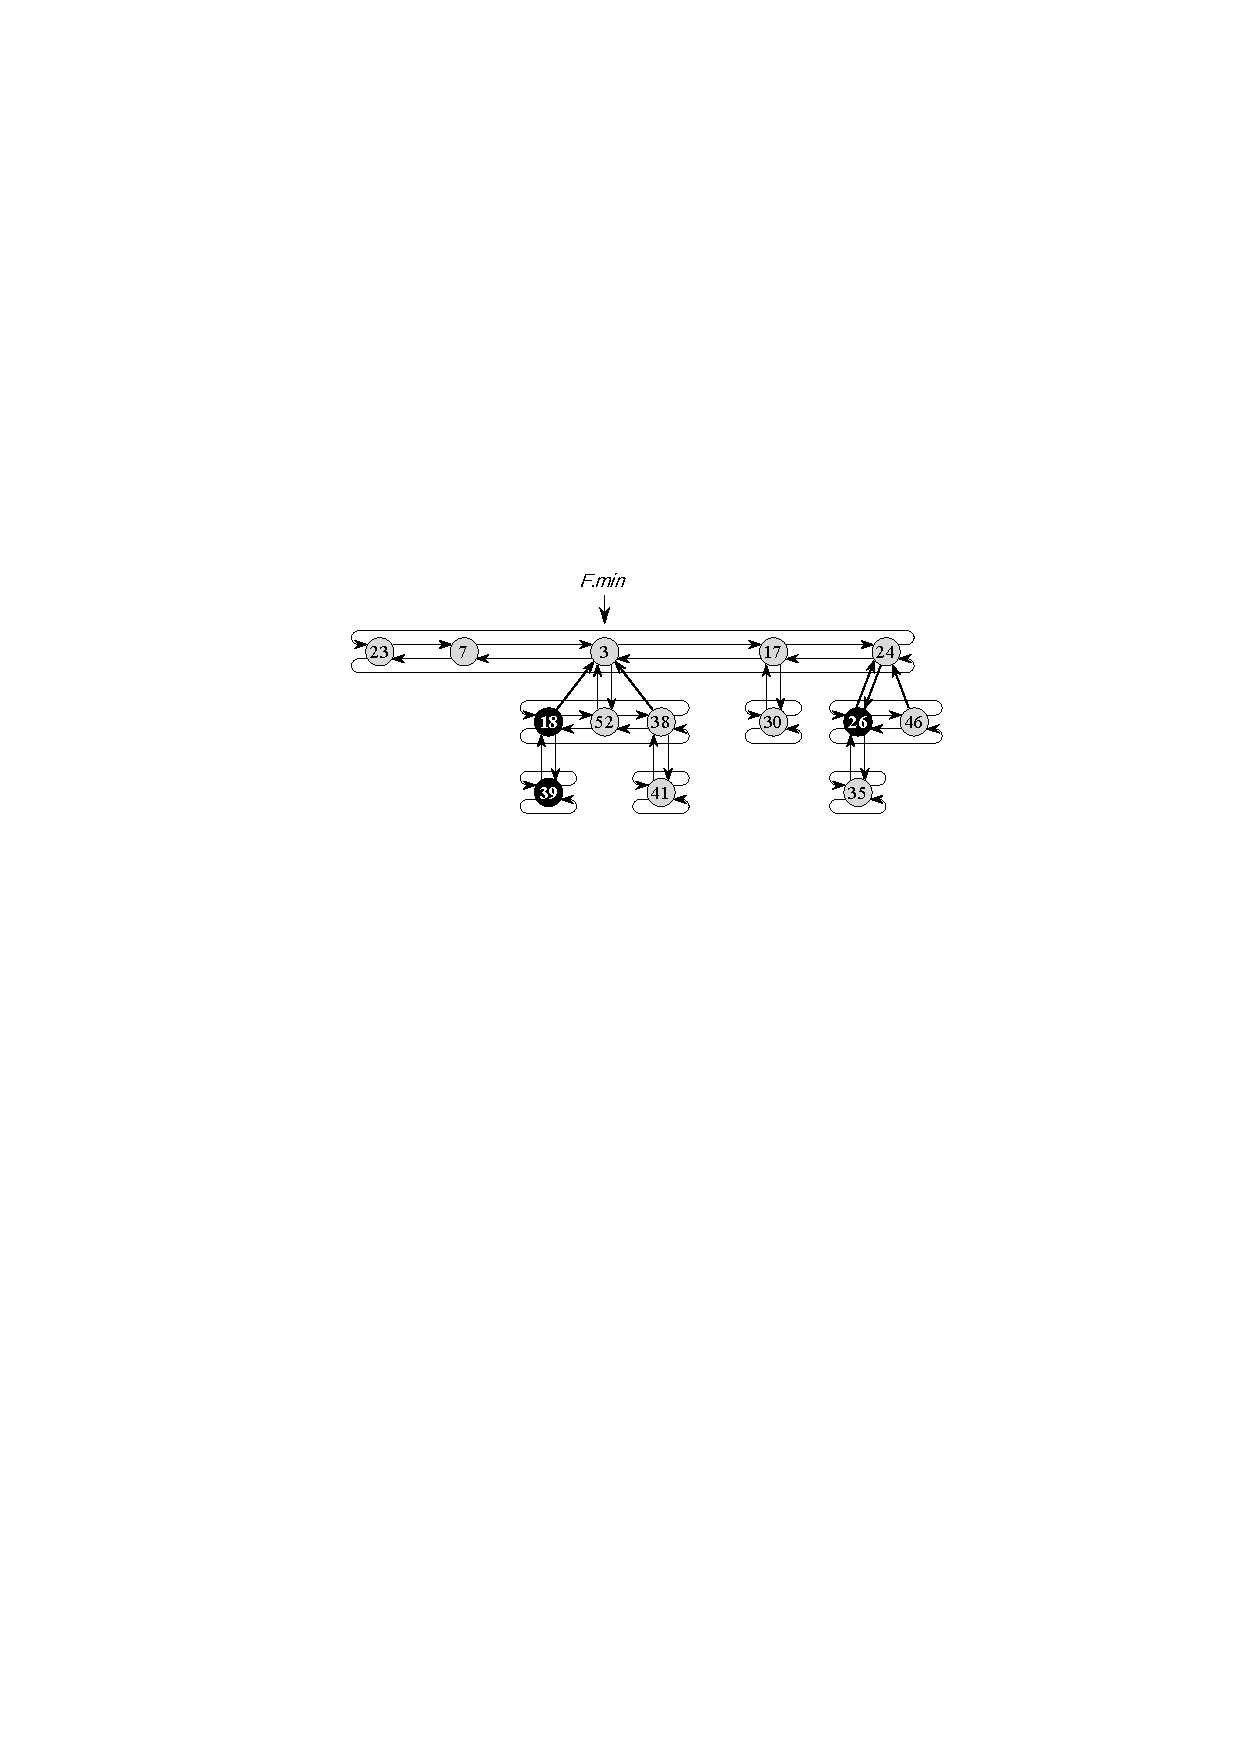
\includegraphics{images/Fibheap1.pdf}
	\caption{A Fibonacci Heap with 5 heaps in the rootlist}
\end{figure}
\subsection{Inserting Node}
To insert a node we call the \prb{Fib-Insert} function and in the function the algorithm initiates the node with setting up all the pointers and variables then add the node to the \emph{rootlist}.\parinf

\begin{minipage}{0.45\textwidth}
	\begin{algorithm}[H]
		\DontPrintSemicolon
		\caption{\textsc{Fib-Create-Node}$(v)$}
		$x.\emph{degree}\longleftarrow 0$\;
		$x.\emph{parent}\longleftarrow None$\;
		$x.\emph{child}\longleftarrow None$\;
		$x.\emph{lost}\longleftarrow 0$\;
		$x.\emph{key}\longleftarrow v$\;
		\Return{$x$}
	\end{algorithm}
\end{minipage}\hfill
\begin{minipage}{0.45\textwidth}
	\begin{algorithm}[H]
		\DontPrintSemicolon
		\caption{\textsc{Fib-Insert}$(F,v)$}
		$x\longleftarrow \textsc{Create-Node}(v)$\;
		\If{$F.\min==None$}{
			$F.\emph{rootlist}\longleftarrow [x]$\;
			$F.\min\longleftarrow x$\;
		}
		\Else{
			$F.\emph{rootlist}.\emph{append}(x)$\;
			\If{$x.key<F.\min.key$}{
				$F.min\longleftarrow x$
			}
		}
	\end{algorithm}
\end{minipage}

All of this can be done in $O(1)$ time. Therefore, to insert a node in the Fibonacci heap it takes $O(1)$ time.
\subsection{Union of Fibonacci Heaps}
To unite to Fibonacci heaps $F_1$ and $F_2$ we simply concatenate the root lists of $F_1$ and $F_2$ and then determine the new minimum node.
\begin{algorithm}
	\DontPrintSemicolon
	\caption{\textsc{Fib-Union}$(F_1,F_2)$}
	$F\longleftarrow \textsc{Make-Fib-Heap}$\;
	$F.\min\longleftarrow F_1.\min$\;
	$F.\emph{rootlist}\longleftarrow F_1.\emph{rootlist} ++ F_2.\emph{rootlist}$\;
	\If{$F_2.\min<F_1.\min$}{
		$F.\min\longleftarrow F_2.\min$
	}
	\Return{$F$}
\end{algorithm}
All the operations here can be done in constant time. Hence, \textsc{Fib-Union} takes $O(1)$ time.
\subsection{Extracting the Minimum Node}
The \textsc{Fib-Extract-Min} function extracts the minimum node from the Fibonacci heap $F$ and then rearranges the heap array. It works by first making a root node out of each of the minimum node's children and removing the minimum node from the rootlist. It then consolidates the root list by linking roots of equal degree until at most one root remains of each degree.
\begin{center}
	\begin{minipage}{0.45\textwidth}
		\begin{algorithm}[H]
			\caption{\textsc{Fib-Extract-Min}$(F)$}
			\DontPrintSemicolon
			$z\longleftarrow F.\min$\;
			\If{$z\neq None$}{
				\For{$x\in z.\emph{child}$}{
					$F.\emph{rootlist}.\emph{append}(x)$\;
					$x.\emph{parent}\longleftarrow None$
				}
				Remove $z$ from $F.\emph{rootlist}$\;
				\If{$z==z.\emph{right}$}{
					$F.\min\longleftarrow None$\;
				}
				\Else{
					$F.\min\longleftarrow z.\emph{right}$
					\emph{consolidate}($F$)
				}
			}
			\Return{$z$}
		\end{algorithm}
		\vspace{2.8cm}

		\begin{algorithm}[H]
			\caption{\textsc{Fib-Heap-Link}$(H,y,x)$}
			\DontPrintSemicolon
			Remove $y$ from $F.\emph{rootlist}$\;
			$y.\emph{parent}\longleftarrow x$\;
			$y.\emph{lost}\longleftarrow 0$
		\end{algorithm}
	\end{minipage}\hfill
	\begin{minipage}{0.5\textwidth}
		\begin{algorithm}[H]
			\caption{\textsc{Consolidate}$(F)$}
			\DontPrintSemicolon
			Initialize array $A[0,\dots, D(n)]$ with \emph{None} elements.\;
			\For{$x\in F.\emph{rootlist}$}{
				$d\longleftarrow x.\emph{degree}$\;
				\If{$A[d]==None$}{
					$A[d]\longleftarrow x$
				}
				\While{$A[d]\neq None$}{
					$y\longleftarrow A[d]$\;
					\If{$y.\emph{key}<x.\emph{key}$}{
						Exchange $x$ with $y$
					}
					\emph{Fib-Heap-Link}$(F,y,x)$\;
					$A[d]\longleftarrow None$, $d\longleftarrow d+1$\;
				}
				$A[d]\longleftarrow x$
			}
			$F.\min\longleftarrow None$\;
			\For{$i=0$ to $D$}{
				\If{$A[i]\neq None$}{
					\If{$F.\min==None$}{
						$F.\emph{rootlist}\longleftarrow [A[i]]$, $F.\min\longleftarrow A[i]$\;
					}
					\Else{
						$F.\emph{rootlist}.\emph{append}(A[i])$\;
						\If{$A[i].\emph{key}<F.\min.\emph{key}$}{
							$F.\min\longleftarrow A[i]$
						}
					}
				}
			}
		\end{algorithm}
	\end{minipage}
\end{center}

Here $D(n)$ denotes the maximum degree a node can have after \textsc{Consolidate}. The procedure \textsc{Consolidate} uses an auxiliary array of size $A$ of size $D$ which we will choose later. For each $i\leq D(n)$ it keeps a heap of degree $i$. And if it finds two 
\begin{figure}[h!]
	\centering
	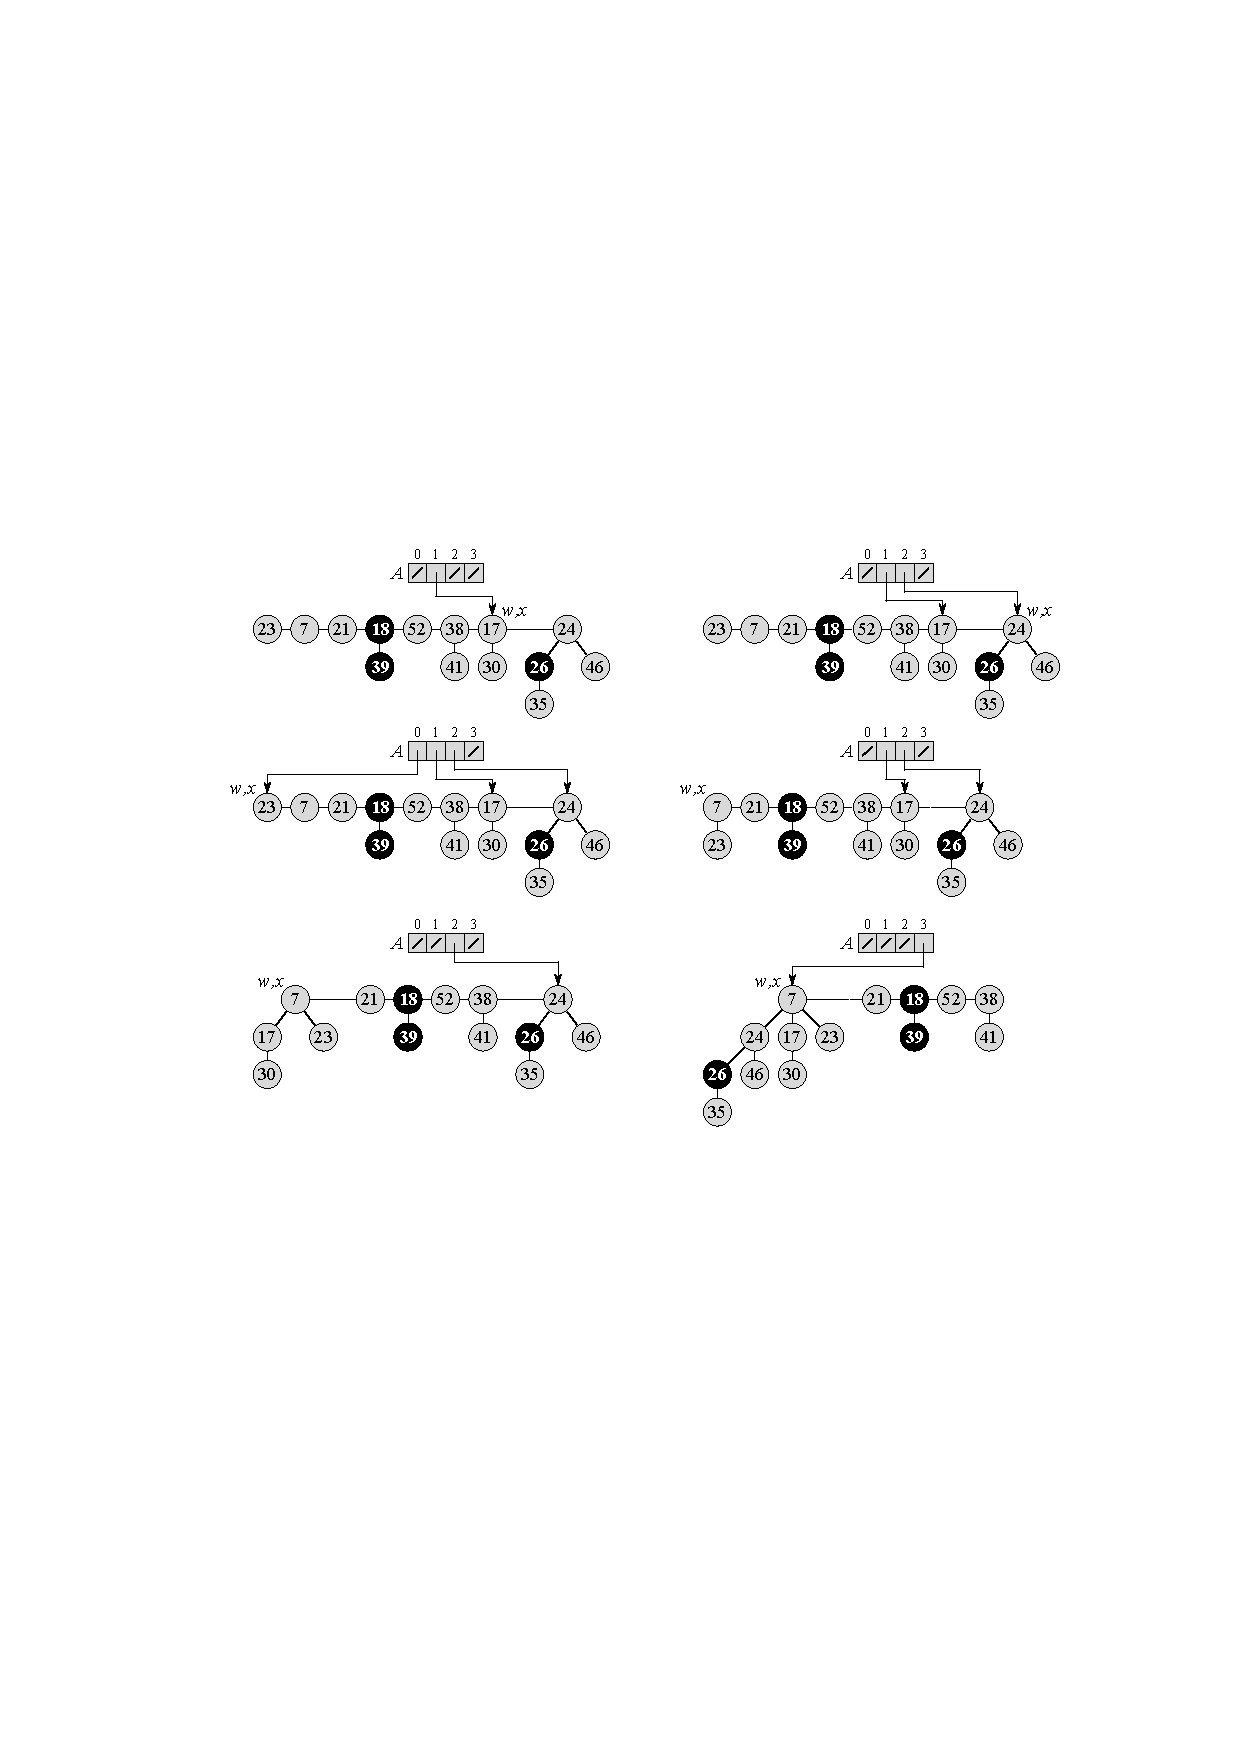
\includegraphics[width=0.75\textwidth]{images/Fibheap2.pdf}
	\caption{A run of \textsc{Consolidate}}
\end{figure}
heaps of same degree then it makes the one with higher key to be the child of the other one. The function \textsc{Fib-Heap-Link} does this process of linking two heaps of same degree.\parinn

Of course in order to allocate array we have to know how to calculate the upper bound for $D(n)$ on the maximum degree. We will show an upper bound of $O(\log n)$ in \autoref{max-degree-bound}.

Now in \textsc{Fib-Extract-Min} in each iteration of the outer for loop or inner while loop it operates on one heap in $F.\emph{rootlist}$. Hence it takes $O(D(n)+\#\text{heaps in $F.\emph{rootlist}$})$ time.


\subsection{Decreasing Key of a Node}
In this section we will show how to decrease a key of a node in a Fibonacci heap in $O(1)$ amortized time. The \textsc{Fib-Decrease-Key} function decreases the key value of the target node then if the min-heap order the node is in is violated then we use the \textsc{Cascading-Cut} function to restore the min-heap property again. These two functions operates like the following:
\begin{center}
	\begin{minipage}{0.45\textwidth}
		\begin{algorithm}[H]
			\caption{\textsc{Fib-Decrease-Key}$(F,x,k)$}
			\DontPrintSemicolon
			\If{$k>x.\emph{key}$}{
				\Return{Error}
			}
			$x.\emph{key}\longleftarrow k$\;
			$y\longleftarrow x.\emph{parent}$\;
			\If{$y\neq None$ and $x.\emph{key}<y.\emph{key}$}{
				\textsc{Cut}$(F,x,y)$\;
				\textsc{Cascading-Cut}$(F,y)$\;
			}
			\If{$k<F.\min.\emph{key}$}{
				$F.\min\longleftarrow x$
			}
		\end{algorithm}
	\end{minipage}\hfill
	\begin{minipage}{0.45\textwidth}
		\begin{algorithm}[H]
			\caption{\textsc{Cascading-Cut}$(F,y)$}
			\DontPrintSemicolon
			% $z\longleftarrow y.\emph{parent}$\;
			\If{$y.\emph{parent}\neq None$}{
				\If{$y.\emph{lost}==0$}{
					$y.\emph{lost}\longleftarrow 1$\;
				}
				\Else{
					\textsc{Cut}$(F,y,y.\emph{parent})$\;
					\textsc{Cascading-Cut}$(F,y.\emph{parent})$
				}
			}
		\end{algorithm}
		\begin{algorithm}[H]
			\caption{\textsc{Cut}$(F,x,y)$}
			\DontPrintSemicolon
			Remove $x$ from $y.\emph{child}$\;
			$y.\emph{degree}\longleftarrow y.\emph{degree}-1$\;
			$F.\emph{rootlist}.\emph{append}(x)$\;
			$x.\emph{parent}\longleftarrow None$, $x.\emph{lost}\longleftarrow 0$\;
		\end{algorithm}
	\end{minipage}
\end{center}
After decreasing the key of the target node if the min-heap order has been violated then we start by cutting the link between $x$ and its parent by adding it to the rootlist. Let $x$ is a node in $F$. At some time $x$ was a root. 
\begin{figure}[h!]
	\centering
	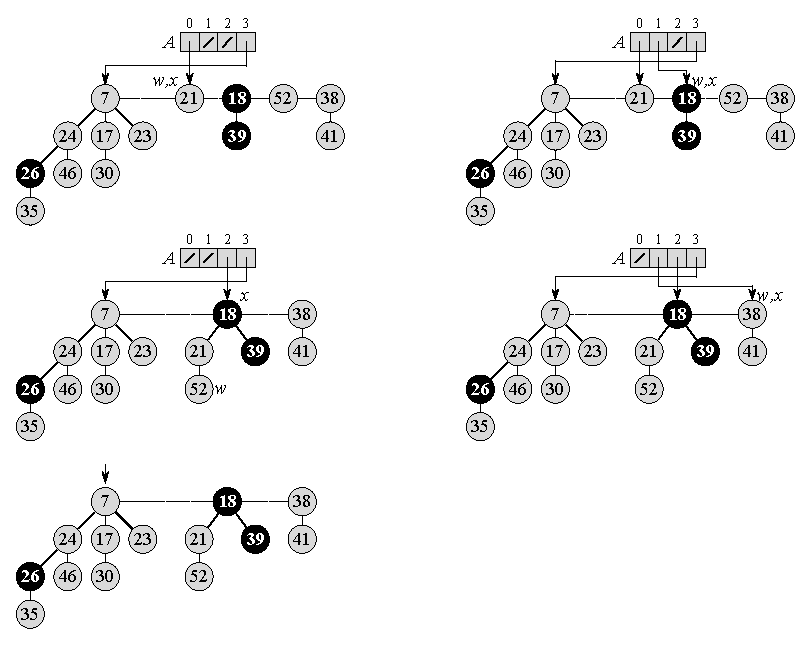
\includegraphics[width=0.7\textwidth]{images/Fibheap3.pdf}
	\caption{A run of \textsc{Cascading-Cut}}
\end{figure}Then $x$ was linked to another node. Suppose at some time two children of $x$ were removed by cuts. As soon as second child has been lost we cut $x$ from its parent and make it a new root. But we are not done yet. Since $x$ might be the second child cut from its parent. So we have to check for its parent. Therefore, we recursively run \textsc{Cascading-Cut} on its parent till we reach the root or cut the first child from a node.

Notice at each run of \textsc{Cascading-Cut} the \emph{lost} bit of a node is getting reset. Therefore, the total time taken by \textsc{Fib-Decrease-Key} is $O(1+\#\text{lost bits reset})$.
\subsection{Bounding the Maximum Degree}\label{max-degree-bound}
To prove that the amortized time of \textsc{Fib-Extract-Min} and \textsc{Fib-Delete} is $O(\log n)$ we must show that upper bound of the maximum degree of any node after \textsc{Consolidate} function is $O(\log n)$. In particular, we will show its $\lt\lfloor \log_{\phi}n\rt\rfloor$ where $\phi$ is the golden ratio.
\begin{lemma}{}{}
	Let $x$ be any node in a Fibonacci heap, and suppose that $x.\emph{degree}=k$. Let $y_1,\dots, y_k$ denote the children of $x$ in the order in which they were linked to $x$ from the earliest to the latest. Then $y_1.\emph{degree}\geq 0$ and $y_i.\emph{degree}\geq i-2$ for $i=2,\dots, k$.
\end{lemma}
\begin{proof}
	Obviously $y_1.\emph{degree}\geq 0$. The only function that adds a child to a node is the function \textsc{Consolidate}. Now for $i\geq 2$, $y_i$ was linked to $x$ when all of $y_1,\dots, y_{i-1}$ were children of $x$, and therefore we must have had $x.\emph{degree}\geq i-1$. Because node $y_i$ is linked to $x$ only if $x\emph{degree}=y_i.\emph{degree}$ we must also have $y_i.\emph{degree}\geq i-1$. Since then node $y_i$ has lost at most one child, since it would have been cut from $x$ by \textsc{Cascading-Cut} if it had lost two children. We conclude that $y_i.\emph{degree}\geq i-2$.
\end{proof}
\begin{lemma}{}{}
	Let $x$ be a node in a Fibonacci heap and let $k=x.\emph{degree}$. Then $$\emph{size}(x)\geq F_{k+2}\geq \phi^k$$
\end{lemma}
\begin{proof}
	We will prove this using induction. For $k=0$, $F_2=1$ so this is obviously true. For $k=1$ there is one child of $x$. Hence, $\emph{size}(x)=2=F_3$. Suppose this is true for $1,\dots, k-1$. Let $y_1,\dots, y_k$ are the children of $x$  in the order in which they were linked to $x$. By the above lemma we have $y_1.\emph{degree}\geq 0$ and $y_i.\emph{degree}\geq i-2$ for all $i=2,\dots, k$. Hence, by Induction hypothesis we have $\emph{size}(y_i)\geq F_{i-2}$ for all $i=2,\dots, k$. Therefore, \[
		\emph{size}(x) \geq 1+\sum\limits_{i=1}^{k}\emph{size}(y_k)\geq 2+\sum\limits_{i=2}^kF_{k}=1+\sum\limits_{i=0}^k F_k=F_{k+2}\geq \phi^k
	\]Hence, we have the lemma.
\end{proof}
\begin{corollary}{}{}
	The maximum degree of any node in \textsc{Consolidate}, $D(n)=O(\log n)$.
\end{corollary}
\subsection{Time Complexity Analysis of Dijkstra}

Now we will calculate the amortized time of Dijkstra algorithm. Before that we will calculate the amortized cost of the data structure. Let in an algorithm  \textsc{Fib-Extract-Min} was called $t$ times. Therefore, total cost of all $t$ many \textsc{Fib-Extract-Min} calls is $O(t\log n+\text{total $\#$heaps created})$. Now heaps are created because of \textsc{Fib-Extract-Min} functions and \textsc{Fib-Decrease-Key} function. We know \textsc{Fib-Extract-Min} were called $t$ times and each time it created $O(\log n)$ heaps. Hence, in total \textsc{Fib-Extract-Min} created $O(t\log n)$ heaps. Therefore, time taken by the $t$ many \textsc{Fib-Extract-Min} calls is $O(t\log n+\#\textsc{Fib-Decrease-Key}\text{ calls})$.

Now suppose in an algorithm $k$ times the function \textsc{Fib-Decrease-Key} function were called. Hence, this takes $O(k+\#\text{total number of \textsc{lost} bits reset})=O(k+\#\text{total number of \textsc{lost} bits rset})$ time. Now the \emph{lost} bits are set only by the \textsc{Fib-Decrease--Key}. Therefore, $\#\text{total number of \textsc{lost} bits rset}=\#\text{\textsc{Fib-Decrese-Key} was called}$. Therefore, the total time taken by all the \textsc{Fib-Decrese-Key} calls is $O(k)$.

Hence, in an algorithm if $t$ times \textsc{Fib-Extract-Min} was called and $k$ times \textsc{Fib-Decrese-Key} was called then total time taken by \textsc{Fib-Extract-Min} is $O(t\log n+k)$ and total time taken by \textsc{Fib-Decrese-Key} is $O(k)$. Therefore, amortized time taken by \textsc{Fib-Extract-Min} is $O(\frac{t}{k}\log n)$ and by \textsc{Fib-Decrese-Key} is $O(1)$.

Now in the Dijkstra algorithm \textsc{Fib-Extract-Min} is called $n$ times and \textsc{Fib-Decrese-Key} is called $O(m)$ times where $n$ is the number of vertices in the graph and $m$ is the number of edges in the graph. Hence, the amortized cost of \textsc{Fib-Extract-Min} is $O(\log n)$ and \textsc{Fib-Decrease-Key} is $O(1)$. Therefore, using Fibonacci heap Dijkstra takes $(n\log n+m)$ time.
